\textbf{TODO: Summary by Anton}
%%% Local Variables:
%%% mode: latex
%%% TeX-master: "../../report"
%%% End:
\begin{figure}[h]
    \centering
    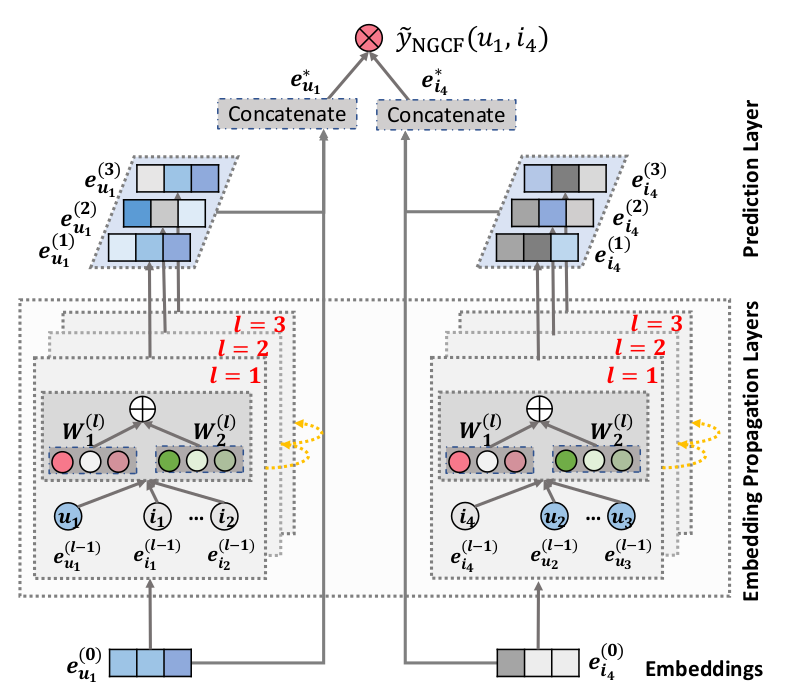
\includegraphics[width=0.8\linewidth]{images/ngcf.png}
    \caption{NGCF architecture.}
    \label{fig:ngcf}
\end{figure}

Tha main difference of NGCF \cite{wang2019neural} and NCF is the ``embedding propagation layers'', which are 
designed to incorporate collaborative signals.
\todo[inline]{Correct next senctence}
This signals include high-order connectivities in users-items connections graph, into embeddings of users and items \ref{fig:ngcf}.
\todo[inline]{TODO Stop}
Therefore, this is supposed to improve the quality of recommendations. 
Each layer corresponds to a measure of the distance between user and item interaction.
It produces messages which are passed between these graph nodes, summed and
\todo[inline]{change: result in embedding at this level.}
In the end all the embeddings for each level are concatenated in order to produce a final embedding.
\todo[inline]{Is this embedding plural or singular? in the next sentence}
This embedding plays the role of latent vectors which can simply be multiplied in order to obtain the rating.
The model is trained using pairwise BPR loss and optimized using Adam.